\begin{frame}[fragile]{On-the-Fly Parameterization (OTFP) to Get $F$ from TAMD}
\begin{tikzpicture}[scaleall=1.0]
\pcuad{\textwidth}{\textheight}
%\showcuad
\path(nw) ++(-0.75,0.0) node(text)[anchor=north west,text 
width=\textwidth]{{\tiny \textcolor{red!80!black}{CFA and E. Vanden-Eijnden 
{\em Chem Phys Lett} {\bf 547}:114 (2012)}}};
\path(c2) ++(-2.5,1.5) node(text)[anchor=north west,text 
width=\textwidth]{\textcolor{blue}{Basis-function expansion}};
\path(c2) ++(-2.5,1.0) node(text)[anchor=north west,text width=\textwidth]{$\ds 
\tilde{F}(\zb) = \sum_k\lambda_k\phi_k(\zb)$};
\path(c1) ++(-2,1.25) node(text)[anchor=north west,text 
width=\textwidth]{\textcolor{blue}{Error as objective function}};
\path(c1) ++(1,-1) node(text)[anchor=north west,text 
width=\textwidth]{\textcolor{blue}{Minimize}};
\path(c1) ++(1,-1.75) node(text)[anchor=north west,text width=\textwidth]{$\ds 
\frac{\partial E}{\partial \lambdab}=0$};
\path(c1) ++(-3.75,0.75) node(text)[anchor=north west,text 
width=\textwidth]{$\ds E(\lambdab) = \Big< 
\sum_j\left[\kappa[z_j-\theta_j(\xb)]-\frac{\partial \tilde{F}(\zb)}{\partial 
z_j}\right]^2\Big>_{\rm TAMD}$};
\path(cp) ++(1.5,.25) node(text)[anchor=north west,text width=\textwidth]{$\ds 
\uu{A}\lambdab = \uu{b}$};
\path(hl) ++(-2.5,1.25) node(text)[anchor=north west,text width=\textwidth]{$\ds 
A_{nm} = \frac{1}{2}\left<\sum_i\frac{\partial \phi_m(\zb)}{\partial z_i} 
\frac{\partial \phi_n(\zb)}{\partial z_i}\right>_{\rm TAMD}$};
\path(hl) ++(-2.5,-0.25) node(text)[anchor=north west,text 
width=\textwidth]{$\ds b_{m} = \left<\sum_i\frac{\partial \phi_m(\zb)}{\partial 
z_i} \kappa[z_i-\theta_i(\xb)]\right>_{\rm TAMD}$};
\draw[<->,thick,color=green!80!black] (0.1\bbw,0.1\bbh) -- (0.5\bbw,0.1\bbh);
\draw[->,thick,color=green!80!black] (0.3\bbw,0.1\bbh) -- (0.3\bbw,0.25\bbh);
\draw[thick,color=orange!50!black] (0.4\bbw,0.1\bbh) -- (0.3\bbw,0.2\bbh);
\draw[thick,color=orange!50!black] (0.3\bbw,0.2\bbh) -- (0.2\bbw,0.1\bbh);
\draw[thick,color=green!80!black] (0.2\bbw,0.1\bbh) -- (0.2\bbw,0.08\bbh);
\draw[thick,color=green!80!black] (0.4\bbw,0.1\bbh) -- (0.4\bbw,0.08\bbh);
\draw[thick,color=green!80!black] (0.3\bbw,0.1\bbh) -- (0.3\bbw,0.08\bbh);
\draw (0.3\bbw,0.06\bbh) node {$m$};
\draw (0.2\bbw,0.06\bbh) node {$m-1$};
\draw (0.4\bbw,0.06\bbh) node {$m+1$};
\draw (0.32\bbw,0.15\bbh) node {1};
\draw (0.35\bbw,0.25\bbh) node {$\phi_m$};
\draw [->,thick,color=orange!80!black] (0.7\bbw,0.7\bbh) -- (0.85\bbw,0.55\bbh);
\draw [->,thick,color=orange!90!black] (0.85\bbw,0.5\bbh) -- (0.8\bbw,0.5\bbh);
\path(c4) ++(-1.0,1.5) node(text)[anchor=north west,text width=\textwidth]{MD vs OTFP: Butane C$_1$-C$_4$\\ Distance Free Energy};
\path(c4) ++(-1.25,0.65) node(corner)[graphics,anchor=north west]{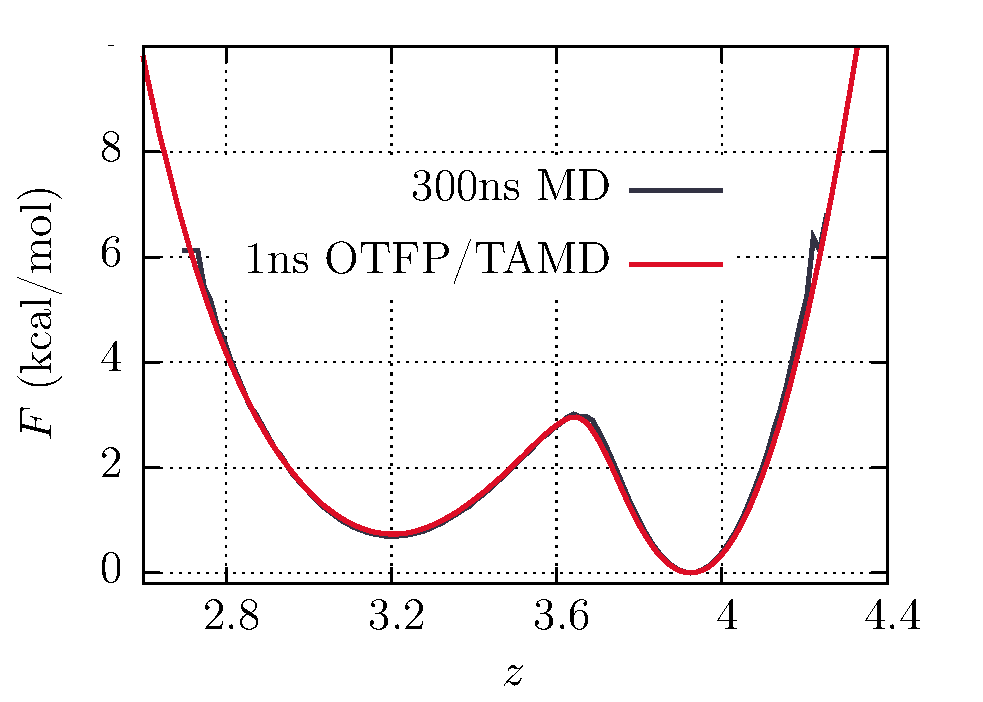
\includegraphics[width=0.33\textwidth]{otfpc4}};
\path(c4) ++(2.25,0.65) node(corner)[graphics,anchor=north west]{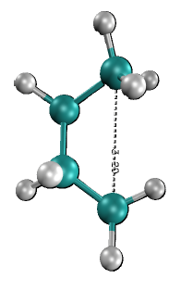
\includegraphics[width=0.1\textwidth]{butane}};
\end{tikzpicture}
\end{frame}

